%************************************************
\chapter{The main theorem}
%************************************************

Let us quickly recall the main theorem we want to prove.

\begin{theorem*}
    A finitely generated right-angled Coxeter group \(W\) has a finite index subgroup \(W'\), such that \(W'\) is residually finite and rationally solvable (RFRS).
\end{theorem*}

Before proceeding with the proof, we should make clear what we have to show.
This is essentially the existence of a series of subgroups, satisfying some conditions.
But what does it mean for a general group to be RFRS?\vspace*{-\parskip}


% ***********************************************
\section{How to be RFRS}
% ***********************************************

We shall start by giving the definition, to shed some light onto our goal.
% In this subsection, we introduce the RFRS condition and discuss how to verify it for a group \(G\).

\begin{definition}
    Let \(G\) be a group.
    Then, \(G\) satisfies the RFRS condition, if there is a sequence of subgroups \(G = G_0 > G_1 > \ldots\), satisfying the following conditions.
    \begin{enumerate}
        \item for each \(i\), \(G_i \triangleleft G\) is a normal subgroup of \(G\),
        \item for each \(i\), the index \([G : G_i]\) is finite,
        \item the intersection \(\bigcap_i G_i\) is the trivial group and
        \item for each \(i\), \((G_i)_r^{(1)} := \ker\{G_i \to \Q \otimes_\Z (G_i)_{\text{ab}}\}\) is a subgroup of \(G_{i+1}\).
    \end{enumerate}
\end{definition}

Observe that in practice, it suffices to show that conditions \(2\) to \(4\) hold. % as once they are satisfied we can simply pass to the Core of each \(G_i\) in \(G\) and this new sequence will.
To see this, let \(G = G_0 > G_1 > \ldots\) be a cofinal sequence of finite index subgroups \(G > G_i\) with \((G_i)_r^{(1)} \leq G_{i+1}\).
Then, for each \(i\) we pass to the core of \(G_i\), given by Core\((G_i) := \bigcap_{g \in G} g G_i g^{-1}\).
By construction the core of a subgroup \(G_i\) is normal in \(G\) and furthermore, we claim the following.
\Claimm{If \(G_i\) has finite index in \(G\), its core will also have finite index in \(G\).}
\Claimmproof{
    Let \(G_i\) be a subgroup in \(G\) with \([G : G_i] < \infty\).
    Then, \(G\) acts (by left multiplication) on the left cosets of \(G_i\) in \(G\) and the kernel of this action consists of the \(h \in G\) with
    \[hgG_i = gG_i \iff g^{-1}hgG_i = G_i \iff g^{-1}hg \in G_i \iff h \in gG_ig^{-1} \quad \forall g \in G.\]
    We note that the kernel is exactly the core of \(G_i\).
    Moreover, the quotient \(\faktor{G}{\text{Core}(G_i)}\) embeds into the symmetric group Sym\((\faktor{G}{G_i})\), whose order is \([G : G_i]!\).
    Thus, we see that if \(G_i\) has finite index in \(G\), the core has finite index as well.
}
So, it remains to check that \((\text{Core}(G_i))_r^{(1)}\) is a subgroup of the group Core\((G_{i+1})\).
Clearly,  for \(g \in G\) we have the equality \(g((G_i)_r^{(1)})g^{-1} = (gG_ig^{-1})_r^{(1)}\), from which we obtain
\[(\text{Core}(G_i))_r^{(1)} \leq \bigcap_{g \in G} (gG_ig^{-1})_r^{(1)} = \bigcap_{g \in G} g(G_i)_r^{(1)}g^{-1} \leq \bigcap_{g \in G} gG_{i+1}g^{-1} = \text{Core}(G_{i+1}).\]
% We conclude that we can omit the first condition in the RFRS condition if we accept to pass to the core of each subgroup \(G_i\) and obtain the sequence \(G \triangleright \text{Core}(G_0) \triangleright \text{Core}(G_1) \triangleright \ldots\;\).
We see that if we are willing to pass to the sequence of core subgroups, we can drop the first condition in the definition of the RFRS condition.

\begin{remark}\label{rmk:tensoring}
    Note that tensoring an abelian group \(A\) (as \(\Z\)-module) with the rationals, `kills' the torsion part of \(A\), whence \(\Q \otimes_\Z A \cong \faktor{A}{\text{Torsion}}\).
    Take for example an elementary tensor \(r \otimes a\) in \(\Q \otimes_\Z A\) so that \(a\) is torsion with order \(n\).
    Then we calculate
    \[r \otimes a  = r \cdot \frac{n}{n} \otimes a = r \cdot \frac{1}{n} \otimes n\cdot a = \frac{r}{n} \otimes a^n = 0.\]
    In particular, for the abelianization \(G_{\text{ab}}\), the group \(\Q \otimes_\Z G_{\text{ab}}\) is isomorphic to the torsion free abelianization \(\faktor{G_{\text{ab}}}{\text{Torsion}}\) and the so called rational derived subgroup \((G)_r^{(1)}\) is the kernel of the homomorphism to the torsion-free abelianization.
\end{remark}


% ***********************************************
\section{Construction of the manifold cover}
% ***********************************************

Consider the abelianization \(W_{\text{ab}}\) of \(W\), which is isomorphic to \((\Z/2\Z)^{n}\).
Now, the abelianization yields a homomorphism \(\alpha : W \to W_{\text{ab}}\) to whose kernel \(\ker\alpha\), we will turn our attention to in the following.
Note that by the first homomorphism theorem, \(\ker\alpha\) has finite index in \(W\), since
\[\abs{\faktor{W}{\ker\alpha}} = \abs{\faktor{\Z}{2\Z}}^{n} = 2^{n} < \infty.\]
Here we used the fact that \(W\) is finitely generated, whence \(n = \abs{I} = \abs{S} < \infty\).

Furthermore, note that for each \(J \subset I\) with \(W_J\) finite, we have an isomorphism between \(W_J\) and \((\faktor{\Z}{2\Z})^{\abs{J}}\).
Thus, the restriction of \(\alpha\) to each such subgroup \(\alpha\vert_{W_J}\) is an injective homomorphism.
We now use that in the right-angled case, the isotropy subgroups of codimension-\(k\) faces are all of this form.
This can be seen, as the isotropy subgroup of a codimension-\(k\) face \(F\) is generated by the reflections in the \(k\) codimension-\(1\) faces, whose intersection forms \(F\).
As all these codimension-\(1\) faces meet at angle \(\frac{\pi}{2}\), the generators commute pairwise.
Therefore, all isotropy subgroups inject into the abelianization of \(W\).
This implies that the intersection of an isotropy subgroup with the kernel of \(\alpha\) is trivial and consequently no isotropy group is contained in the kernel \(\ker\alpha\).
Since finite subgroups are contained in isotropy subgroups, the kernel \(\ker\alpha\) acts freely on the Tits cone \(WC\) corresponding to \(W\).

In particular, by \Cref{thm:stabilizer} the action of \(W\) on the interior of its Tits cone \(int(WC)\) is properly discontinuously.
By \Cref{thm:convexity} the Tits cone is also a convex cone, implying that it has trivial fundamental group, whence is simply-connected.
Having all this information, we are able to apply \Cref{lem:covering} to obtain the covering
\[int(WC) \;\longrightarrow\; \faktor{int(WC)}{\ker\alpha} \qquad x \mapsto \text{Orb}_{\ker\alpha}(x).\]
% Using the local homeomorphism property of a covering map and the fact that the Tits cone \(WC\) is a subspace of \(\R^n\), we conclude that the quotient \(\faktor{int(WC)}{\ker\alpha}\) is indeed a manifold.
We conclude the results of this section in the following proposition.

\begin{proposition}
    Let \(W\) be a right-angled Coxeter group with corresponding Tits cone \(WC\). % and fundamental chamber \(C\).
    Then, there is a finite index subgroup \(W' \leq W\), acting by covering action on the interior of the Tits cone, implying that the quotient \(\faktor{int(WC)}{W'}\;\) is a manifold.
    In particular, \(W' = \ker\{W \to W_{\text{ab}}\} = \ker\alpha\).
    % In particular, we can take \(W'\) to be the kernel of the abelianization homomorphism \(\alpha : W \to W_{\text{ab}}\).
\end{proposition}


% ***********************************************
\section{Some orbifold theory}
% ***********************************************

In this section, we want to elaborate more on the natural orbifold structure of the fundamental chamber \(C\).
We start by giving a formal definition of an orbifold.
We break the definition down into smaller pieces, starting with local models, sometimes called (orbifold) charts.

\begin{definition}
    A \emph{local model} is a pair \((\widetilde{U}, \Gamma)\), where \(\widetilde{U} \subset \R^n\) is open and \(\Gamma\) is a finite subgroup of the group of diffeomorphisms of \(\widetilde{U}\), denoted \emph{diffeo}\((\widetilde{U})\), acting on \(\widetilde{U}\).
    By abusing notation, we will sometimes say that the quotient \(U = \faktor{\widetilde{U}}{\Gamma}\;\) is the local model.
\end{definition}

Now that we have defined the local structure of an orbifold, we want to translate between these local models.
This is being made precise by orbifold maps.

\begin{definition}
    An \emph{orbifold map} between local models \((\widetilde{U}_i, \Gamma_i), (\widetilde{U}_j, \Gamma_j)\) is a pair of maps \((\widetilde{\psi}, \varphi)\),
    consisting of a smooth map \(\widetilde{\psi} : \widetilde{U}_i \to \widetilde{U}_j\) and a homomorphism of groups \(\varphi : \Gamma_i \to \Gamma_j\).
    We enforce the map \(\widetilde{\psi}\) to be \(\varphi\)-equivariant, meaning that for all \(g \in \Gamma_i\) and all \(\widetilde{x} \in \widetilde{U}_i\), \(\widetilde{\psi}(g\widetilde{x}) = \varphi(g)\widetilde{\psi}(\widetilde{x})\) holds.
    Then \(\widetilde{\psi}\) induces a map \(\psi : \faktor{\widetilde{U}_i}{\Gamma_i} \to \faktor{\widetilde{U}_j}{\Gamma_j}\), between the local models.
    When all three of these maps are injective, we call \(\psi\) a local isomorphism.
\end{definition}

Now that we have these local definitions, we `glue' them together, to obtain an orbifold.
Before we do so, we recall some notions from topology.

Suppose, we are given an open cover \(\{U_i\}\) of a topological space \(X\).
It is said to be \emph{locally finite}, if every \(x \in X\) admits a neighborhood \(N\) such that \(N \cap U_i\) is empty for all but finitely many \(i\).
The open cover \(\{U_i\}\) is a \emph{refinement} of an open cover \(\{V_j\}\) of \(X\), if for every \(V_j\) there is a \(U_i\) with \(U_i \subseteq V_j\).
Now, the topological space \(X\) is said to be \emph{paracompact}, if every open cover of \(X\) admits such a locally finite refinement.

\begin{definition}
    An \(n\)-dimensional \emph{(smooth) orbifold} \(Q\) is a pair \((X_Q, \mathcal{A})\).
    The space \(X_Q\) is a paracompact Hausdorff space, called the \emph{underlying space}.
    The set \(\mathcal{A}\) is called an \emph{orbifold atlas}, consisting of charts \((U_i, \phi_i)\), indexed by some set \(I\) and satisfying the following conditions:
    \begin{itemize}
        \item the \(U_i\) form an open cover of the underlying space \(X_Q\),\vspace*{-.7em}
        \item for each \(U_i\) there exists a local model \(\faktor{\widetilde{U}_i}{\Gamma_i}\) with a homeomorphism \(\phi_i : U_i \to \faktor{\widetilde{U}_i}{\Gamma_i}\) and
        \item charts have to be compatible, meaning that for \(U_i \subset U_j\) the inclusion is a local isomorphism.
    \end{itemize}
\end{definition}

To sketch the connection between manifolds and orbifolds, let us mention one more thing.

\begin{definition}
    The \emph{local group} \(loc(x)\) of some \(x\) in a local model \(\faktor{\widetilde{U}}{\Gamma}\;\) is the isotropy group of any \(\widetilde{x}\) in \(\widetilde{U}\), getting projected onto \(x\).
    The \emph{singular locus} \(\Sigma (Q)\) of an orbifold \(Q\) consists of all points in the underlying space \(X_Q\) with non-trivial local group, i.e. \(\Sigma(Q) = \{x \in X_Q \;\vert\; loc(x) \neq \{1\}\}\).
\end{definition}

By this definition, we see that an orbifold with empty singular locus is just a manifold.
Furthermore, when thinking about an orbifold, we can just think about the underlying space and label each element in the singular locus by its local group.

Many basic examples arise by taking the quotient relative to a properly discontinuous group action on \(\R^n\).
We want to mention at least some examples.

\begin{example} % TODO: add pictures
    \begin{enumerate}
        \item Consider the flat plane \(\R^2\) with the action of a cyclic group \(\faktor{\Z}{n\Z}\) by rotation about the origin.
            The arising orbifold is a cone with singular point the origin and cone angle \(\frac{2\pi}{n}\).
        
        \item Consider the sphere \(S^2\) with the action of a cyclic group \(\faktor{\Z}{2\Z}\) by rotation about the north pole \(N\).
            The arising orbifold now is called a \emph{teardrop} with singular point, the north pole \(N\).
            
        % \item Cosider the torus \(\mathbb{T}^2 \cong \faktor{\R^2}{\Z^2}\) with the action of the group \(\faktor{\Z}{2\Z}\) acting by reflection in the midpoints of the y-axis of \(\Z^2\)-lattice in \(\R^2\).
    \end{enumerate}
\end{example}

By starting with a topological space \(X\), this is actually a more general way to construct orbifolds.
Given a properly discontinuously action of a group \(G\) on \(X\), simply pass to the quotient space \(\faktor{X}{G}\) to obtain an orbifold.
In contrast, to obtain a manifold, one has to demand the action to be free as well.
This is not the only analogy between manifolds and orbifolds.
The concept of orbifold coverings translates almost one to one from the ordinary case.

\begin{definition}
    An orbifold covering \(p: Q' \to Q\) is a continuous map on the underlying spaces \(X_{Q'} \to X_Q\), such that for each point \(x \in X_Q\) there is a local model \(U = \faktor{\widetilde{U}}{\Gamma}\) around \(x\) and each component \(V_i\) of \(p^{-1}(U)\) is homeomorphic to \(\faktor{\widetilde{U}}{\Gamma_i}\) for a subgroup \(\Gamma_i\) of \(\Gamma\).
    Furthermore, the restriction \(p\vert_{V_i} : V_i \to U\) corresponds to the natural projection \(\faktor{\widetilde{U}}{\Gamma_i} \to \faktor{\widetilde{U}}{\Gamma}\).
\end{definition}

\begin{remark}\label{rmk:covers}
    We want to mention here, that the universal cover of an orbifold is exactly what we think of, i.e. the initial object in the category of orbifold coverings.
    Moreover, there is a notion of orbifold fundamental groups as well and they behave to orbifold covers the same as fundamental groups to coverings in the ordinary case.
    In particular, subgroups (of index \(n\)) of the orbifold fundamental group correspond to (\(n\)-sheeted) orbifold coverings.
\end{remark}
    
Having all this in mind, we have two ways of approaching the fundamental chamber \(C\).
One way, it obtains its natural orbifold structure as the quotient \(\faktor{int(WC)}{W}\).
As the Tits cone is simply connected, it is the universal cover of \(C\) and we observe that the orbifold fundamental group of \(C\) is precisely \(W\).
On the other hand, the fundamental chamber is the quotient of the manifold \(\faktor{int(WC)}{W'}\) by a finite group action.
\vspace*{\parskip}

\begin{figure}[h!]
    \begin{minipage}[c]{.6\textwidth}
        Since \(W'\) is a finite index subgroup of \(W\), \Cref{rmk:covers} implies that we get a covering map \(p\) so that the diagram on the right commutes.
        Thus, both of the approaches to the fundamental chamber \(C\) agree in the sense that the projection map \(int(WC) \to \faktor{int(WC)}{W}\) factors through the manifold cover, constructed in Section \(3.1\).
    \end{minipage}\quad
    \begin{minipage}{.35\textwidth}\vspace*{-1em}
        \begin{tikzcd}
            int(WC) \arrow[r] \arrow[d] & \faktor{int(WC)}{W} \\
            \faktor{int(WC)}{W'} \arrow[ru, "p"', dashed]
        \end{tikzcd}
    \end{minipage}
\end{figure}


% ***********************************************
\section{The cofinal cover}
% ***********************************************

In this section, we want to at least \emph{sketch} the proof of the existence of a cofinal sequence of two-fold covers, arising by iteratively reflecting in faces.
Some more results from the theory of orbifolds are needed for the whole proof.
We will state and use them without proof.

In the following, doubling along a face means the construction of a sequence of polytopes \(P_k = P_{k-1} \cup g_{k-1}(P_{k-1})\), where \(g_{k-1}\) is the reflection in one of the faces of the previous polytope \(P_{k-1}\).
The following proposition will tell us, that in the case of a right-angled Coxeter group, we are able to double the fundamental chamber \(C\) in one of its faces and are still able to cover the whole Tits cone \(WC\) by reflecting in the faces of the resulting chamber.

\begin{proposition}\label{prop:double}
    Let \(P_k \subset \R^n\) be a polytope with orbifold structure, orbifold fundamental group \(\pi_1^{\text{orb}}(P_k)\) and universal cover \(\widetilde{P}\).
    Then, the fundamental group \(\pi_1^{\text{orb}}(P_{k+1})\) is isomorphic to the group generated by reflections in the faces of the double \(P_{k+1}\).
    Furthermore, the fundamental group \(\pi_1^{\text{orb}}(P_{k+1})\) of the double is an index-\(2\) subgroup of \(\pi_1^{\text{orb}}(P_k)\) and the following two conditions are satisfied.
    \begin{enumerate}
        \item \(\forall k \in \N: \forall g \in \pi_1^{\text{orb}}(P_k): g(\mathring{P_k}) \cap \mathring{P_k} \neq \emptyset \implies g = 1\), and
        \item \(\forall k \in \N: \bigcup_{g \in \pi_1^{\text{orb}}(P_k)} g(P_{k}) = \widetilde{P}\).
    \end{enumerate}
\end{proposition}
\begin{proof}
    We won't proof this here.
\end{proof}

To state the other helping lemma we will need, we first want to show that each chamber in the Tits cone can uniquely be labeled by elements of its corresponding group.

\begin{lemma}\label{lem:labels}
    Let \(W\) be a Coxeter group and \(WC\) its Tits cone.
    The chambers of the form \(w(C)\) in the Tits cone can be labeled uniquely by elements in \(W\).
\end{lemma}
\begin{proof}
    Let \(v(C), w(C)\) be chambers in \(WC\) for \(v, w \in W\), such that \(v \neq w\) and \(w(C) = v(C)\).\newline
    But then, by \Cref{thm:stabilizer} we have that
    \[w(\mathring{C}) \cap v(\mathring{C}) = w(\mathring{C} \cap w^{-1}v(\mathring{C})) \neq \emptyset \implies w^{-1}v = 1 \iff w = v.\]
    Thus, the chambers can be labeled in a unique way.
\end{proof}

We proceed with another helpful result, whose proof relies on the aforementioned results.

\begin{lemma}
    Let \(C \subset \R^n\) be the fundamental chamber of a Coxeter group \(W\).
    The non-trivial labels \(w_i \neq 1_W\) of the chambers, defining the polytope \(P = \bigcup_{i=1}^n w_i(C)\), are \emph{not} contained in the reflection group, generated by reflecting in its faces.
\end{lemma}
\begin{proof}
    Note that by \Cref{lem:labels}, the chambers of the form \(w(C)\) are uniquely labeled by \(w \in W\).
    Thus, let \(P := \bigcup_{i = 1}^n w_i(C)\) be as in the lemma and \(w_i\) one of its defining labels.
    Assume, \(w_i \neq 1_W\) is contained in the reflection group generated by reflecting in the faces of \(P\).
    But then we have that \(w_i(\mathring{P}) \cap \mathring{P} \neq \emptyset\), contradicting \Cref{prop:double}.
\end{proof}

Using this insight, we define a graph \(G\) with vertices \(V(G) := \{w(C) \;\vert\; w \in W\}\) and edges \(E(G) := W \times S\).
The endpoint map is given by \(\delta : W \times S \to 2^{V(G)},\; (w, s) \mapsto (w(C), ws(C))\).
Thus, two vertices \(w(C)\) and \(v(C)\) have an edge, if there is an \(s \in S\), such that \(ws = v\).
Then, clearly we have \(wsw^{-1}w(C) = ws(C) = v(C)\).
Note that the element \(wsw^{-1}\) is the only element, that flips the edge \(\{w(C), ws(C)\}\).
Thus, the map \(W \times S \to W, \; (w, s) \mapsto wsw^{-1}\) defines a labeling of the edges by elements in \(W\).
We will call the combinatorial graph of \(G\) (meaning that every double edge gets collapsed) the \emph{chamber graph} Cham\((W, S)\) of \(W\).

It is obvious, that this graph is isomorphic to the combinatorial Cayley graph of the group \(W\) and we see that the Cayley graph `embeds' into the Tits cone \(WC\).
This will be useful to prove the main theorem of this section next.

\begin{theorem}\label{thm:cofinal}
    % By doubling in a face of the fundamental chamber and iteratively doubling the resulting chamber, we will at some point cover every chamber in the Tits cone \(WC\).
    The doubling sequence \(P_k\), starting in the fundamental chamber \(P_0 = C\), is cofinal.
    This means, the chamber \(P_n\) for some \(n\), covers the whole Tits cone.
\end{theorem}
\begin{proof}
    The proof is by induction on the word length \(\ell(w)\).
    For \(\ell(w) = 0\), the corresponding chamber is the fundamental chamber \(C\), which is covered by itself.
    \IH{Chambers with labels \(v\) of length \(\ell(v) = k - 1\) are covered by a polytope \(P = \bigcup_{i=1}^n w_i(C)\).}\par\noindent
    We need to show that chambers of the form \(w(C)\) with \(\ell(w) = k\) can be covered by reflecting in a face of the polytope \(P\).
    Using the chamber graph Cham\((W, S)\), constructed above, we deduce that for each such \(w\), there is a \(v \in W\) of length \(\ell(v) = k - 1\), connected to \(w\) by an edge in Cham\((W, S)\). % , labeled by \(ws_iw^{-1}\) for an \(i \in I\).
    This is due to the fact that the chamber graph is isomorphic to the Cayley graph of  \(W\) and the length function of \(W\) is induced by the Cayley graph.
    But then, the chamber \(w(C)\) is adjacent to the chamber \(v(C)\) and the latter is contained in \(P\) by \textbf{(IH)}.
    Thus, either \(w(C)\) itself is already contained in \(P\) or we reflect in the face shared by \(w(C)\) and \(v(C)\) to cover \(w(C)\) with the double \(P'\) of \(P\).
    Now, continuing with the next element \(w\) of length \(k\), we eventually double \(P'\) and repeat this for all such \(w\).
    This iterative doubling process is valid by \Cref{prop:double} and by induction every chamber \(g(C)\) for \(g \in W\) can be covered.
\end{proof}

% The conclusion of this section is that the doubling sequence starting in the fundamental chamber \(C\) of the right-angled Coxeter group \(W\) is a cofinal sequence of two-fold (orbifold) covers.
% Thus, we conclude that the doubling sequence starting in the fundamental chamber \(C\) is a cofinal sequence of two-fold covers.

\begin{remark}\label{rmk:groupseries}
    Using \Cref{prop:double}, we see that the cofinality of this sequence translates to the group side.
    More precisely, this sequence of two-fold covers induces a sequence of index-\(2\) subgroups via the fundamental groups of the covering spaces.
    As we will at some point cover the whole Tits cone, whose fundamental group is trivial, the intersection of all these groups is trivial.
\end{remark}

% \begin{figure}[ht!]
%     \centering
%     \subfloat[The fundamnetal chamber \(C\).]{{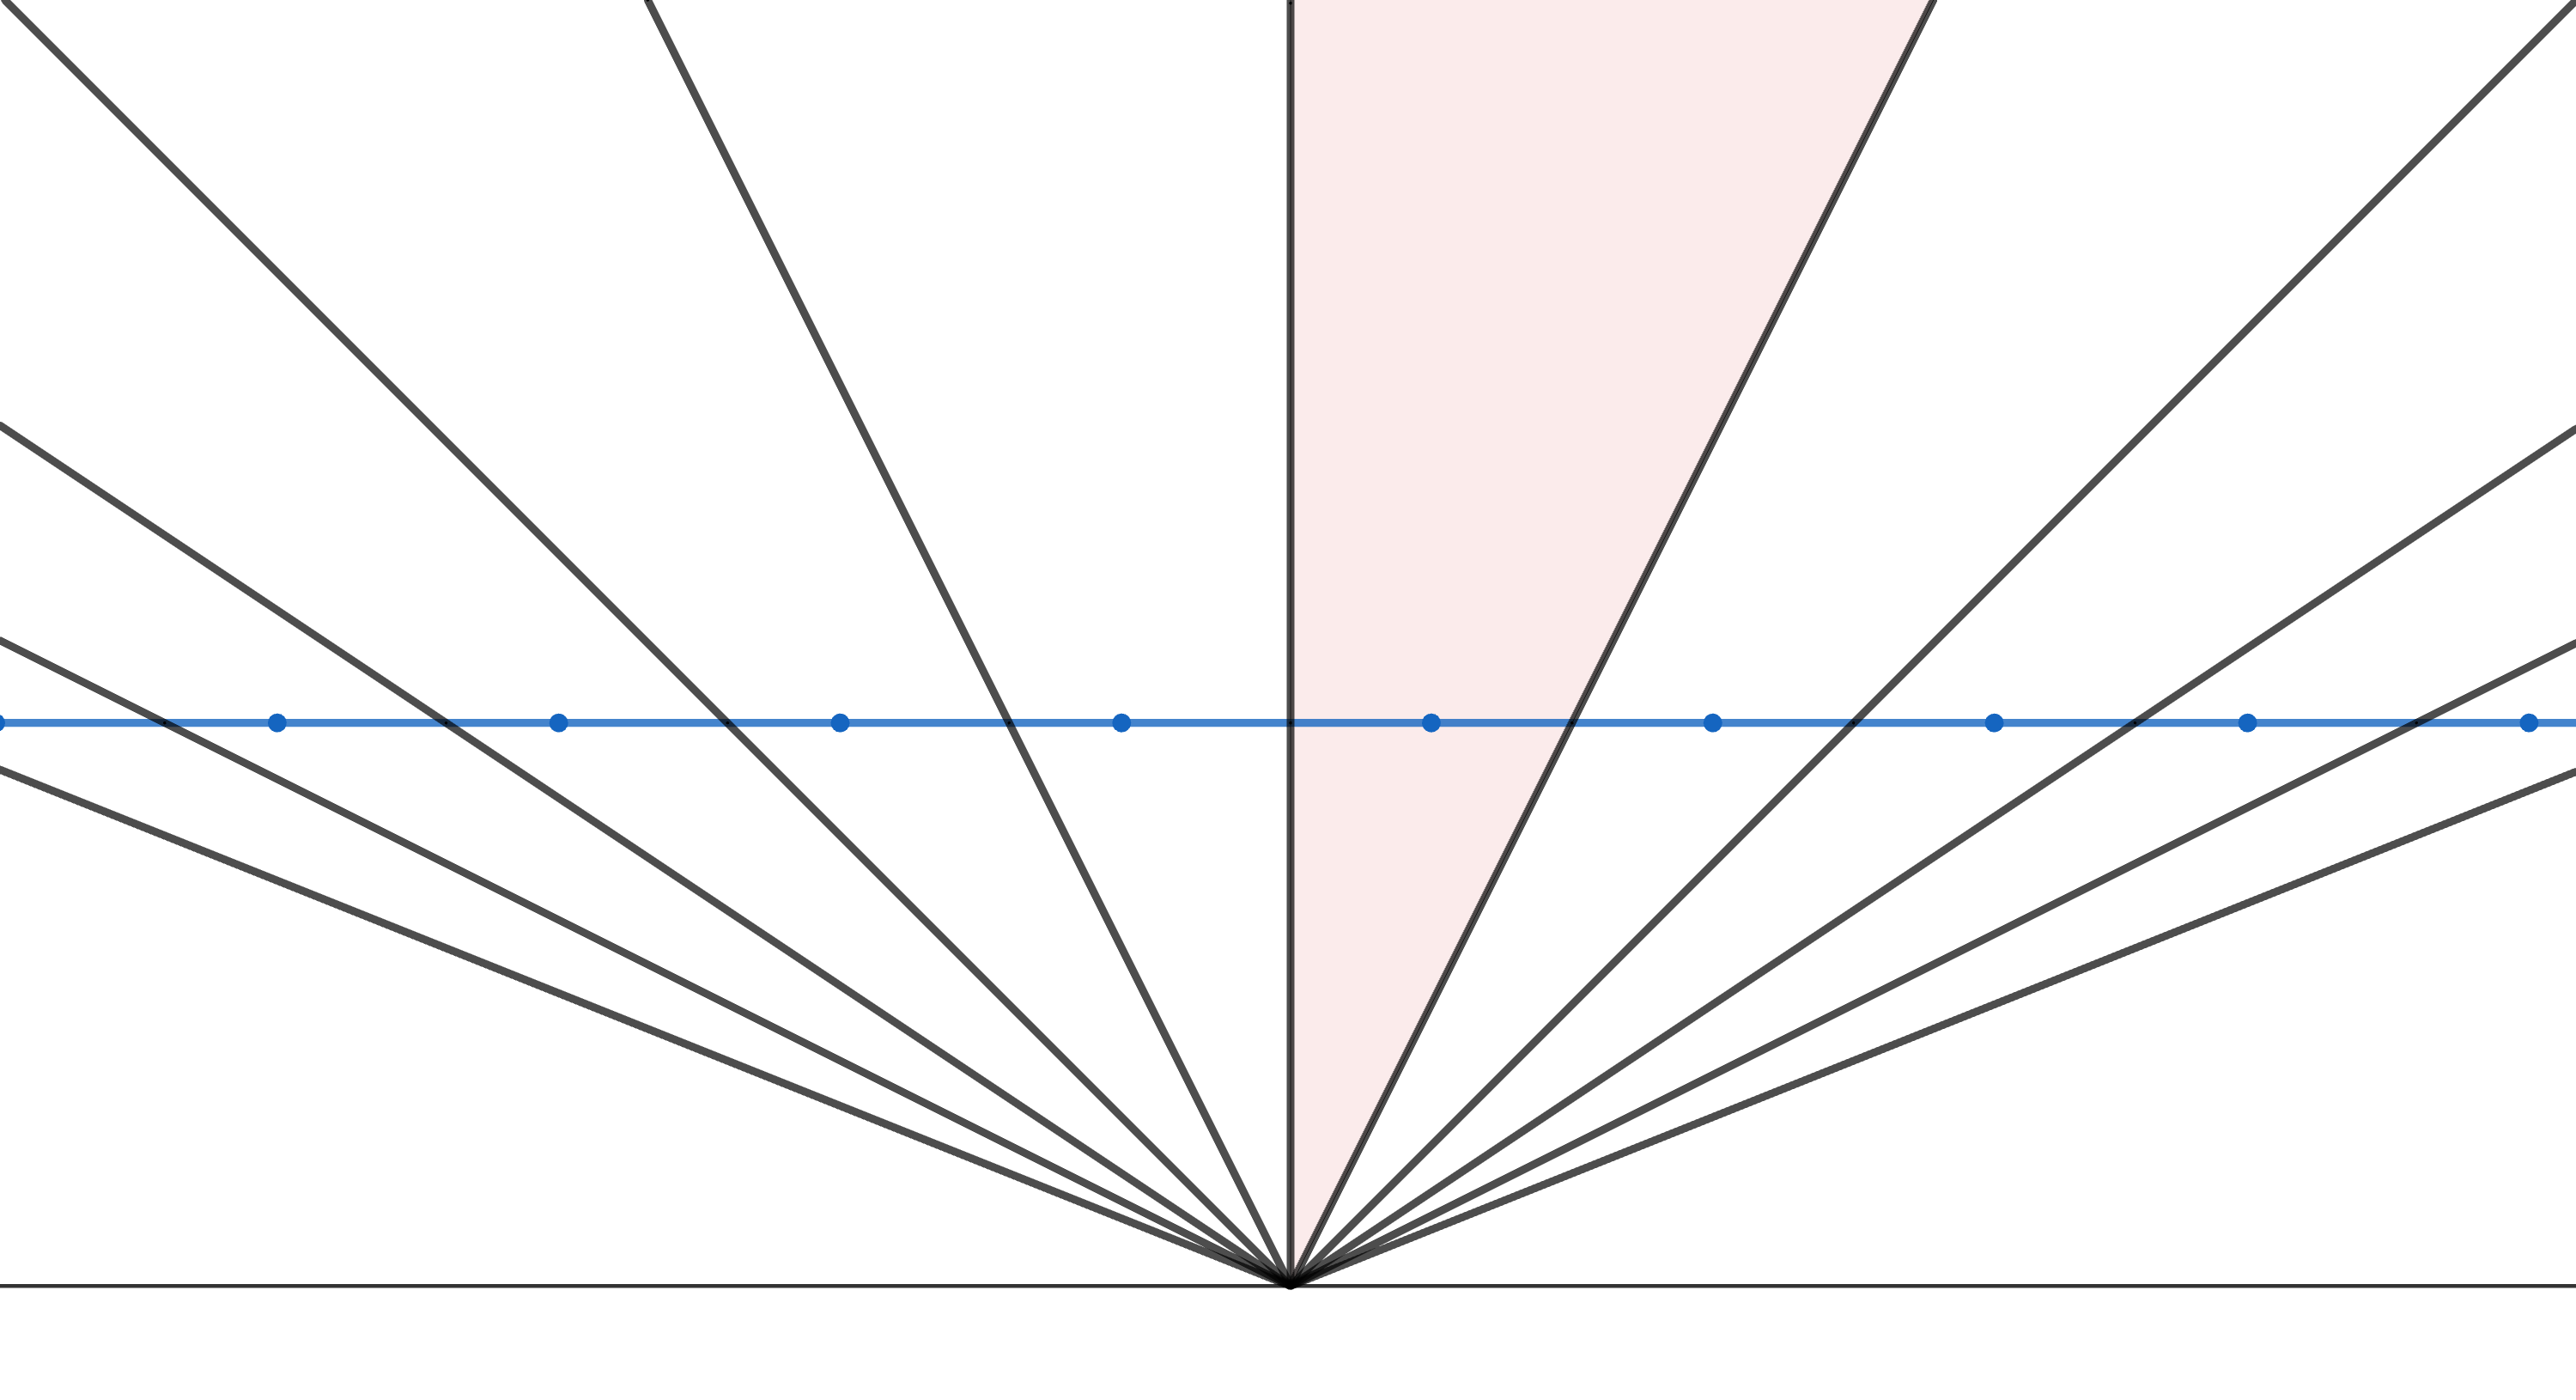
\includegraphics[width=6cm]{gfx/chamber graph - 1.png}}}\qquad
%     \subfloat[The double polytope \(P = C \cup s_1(C)\)]{{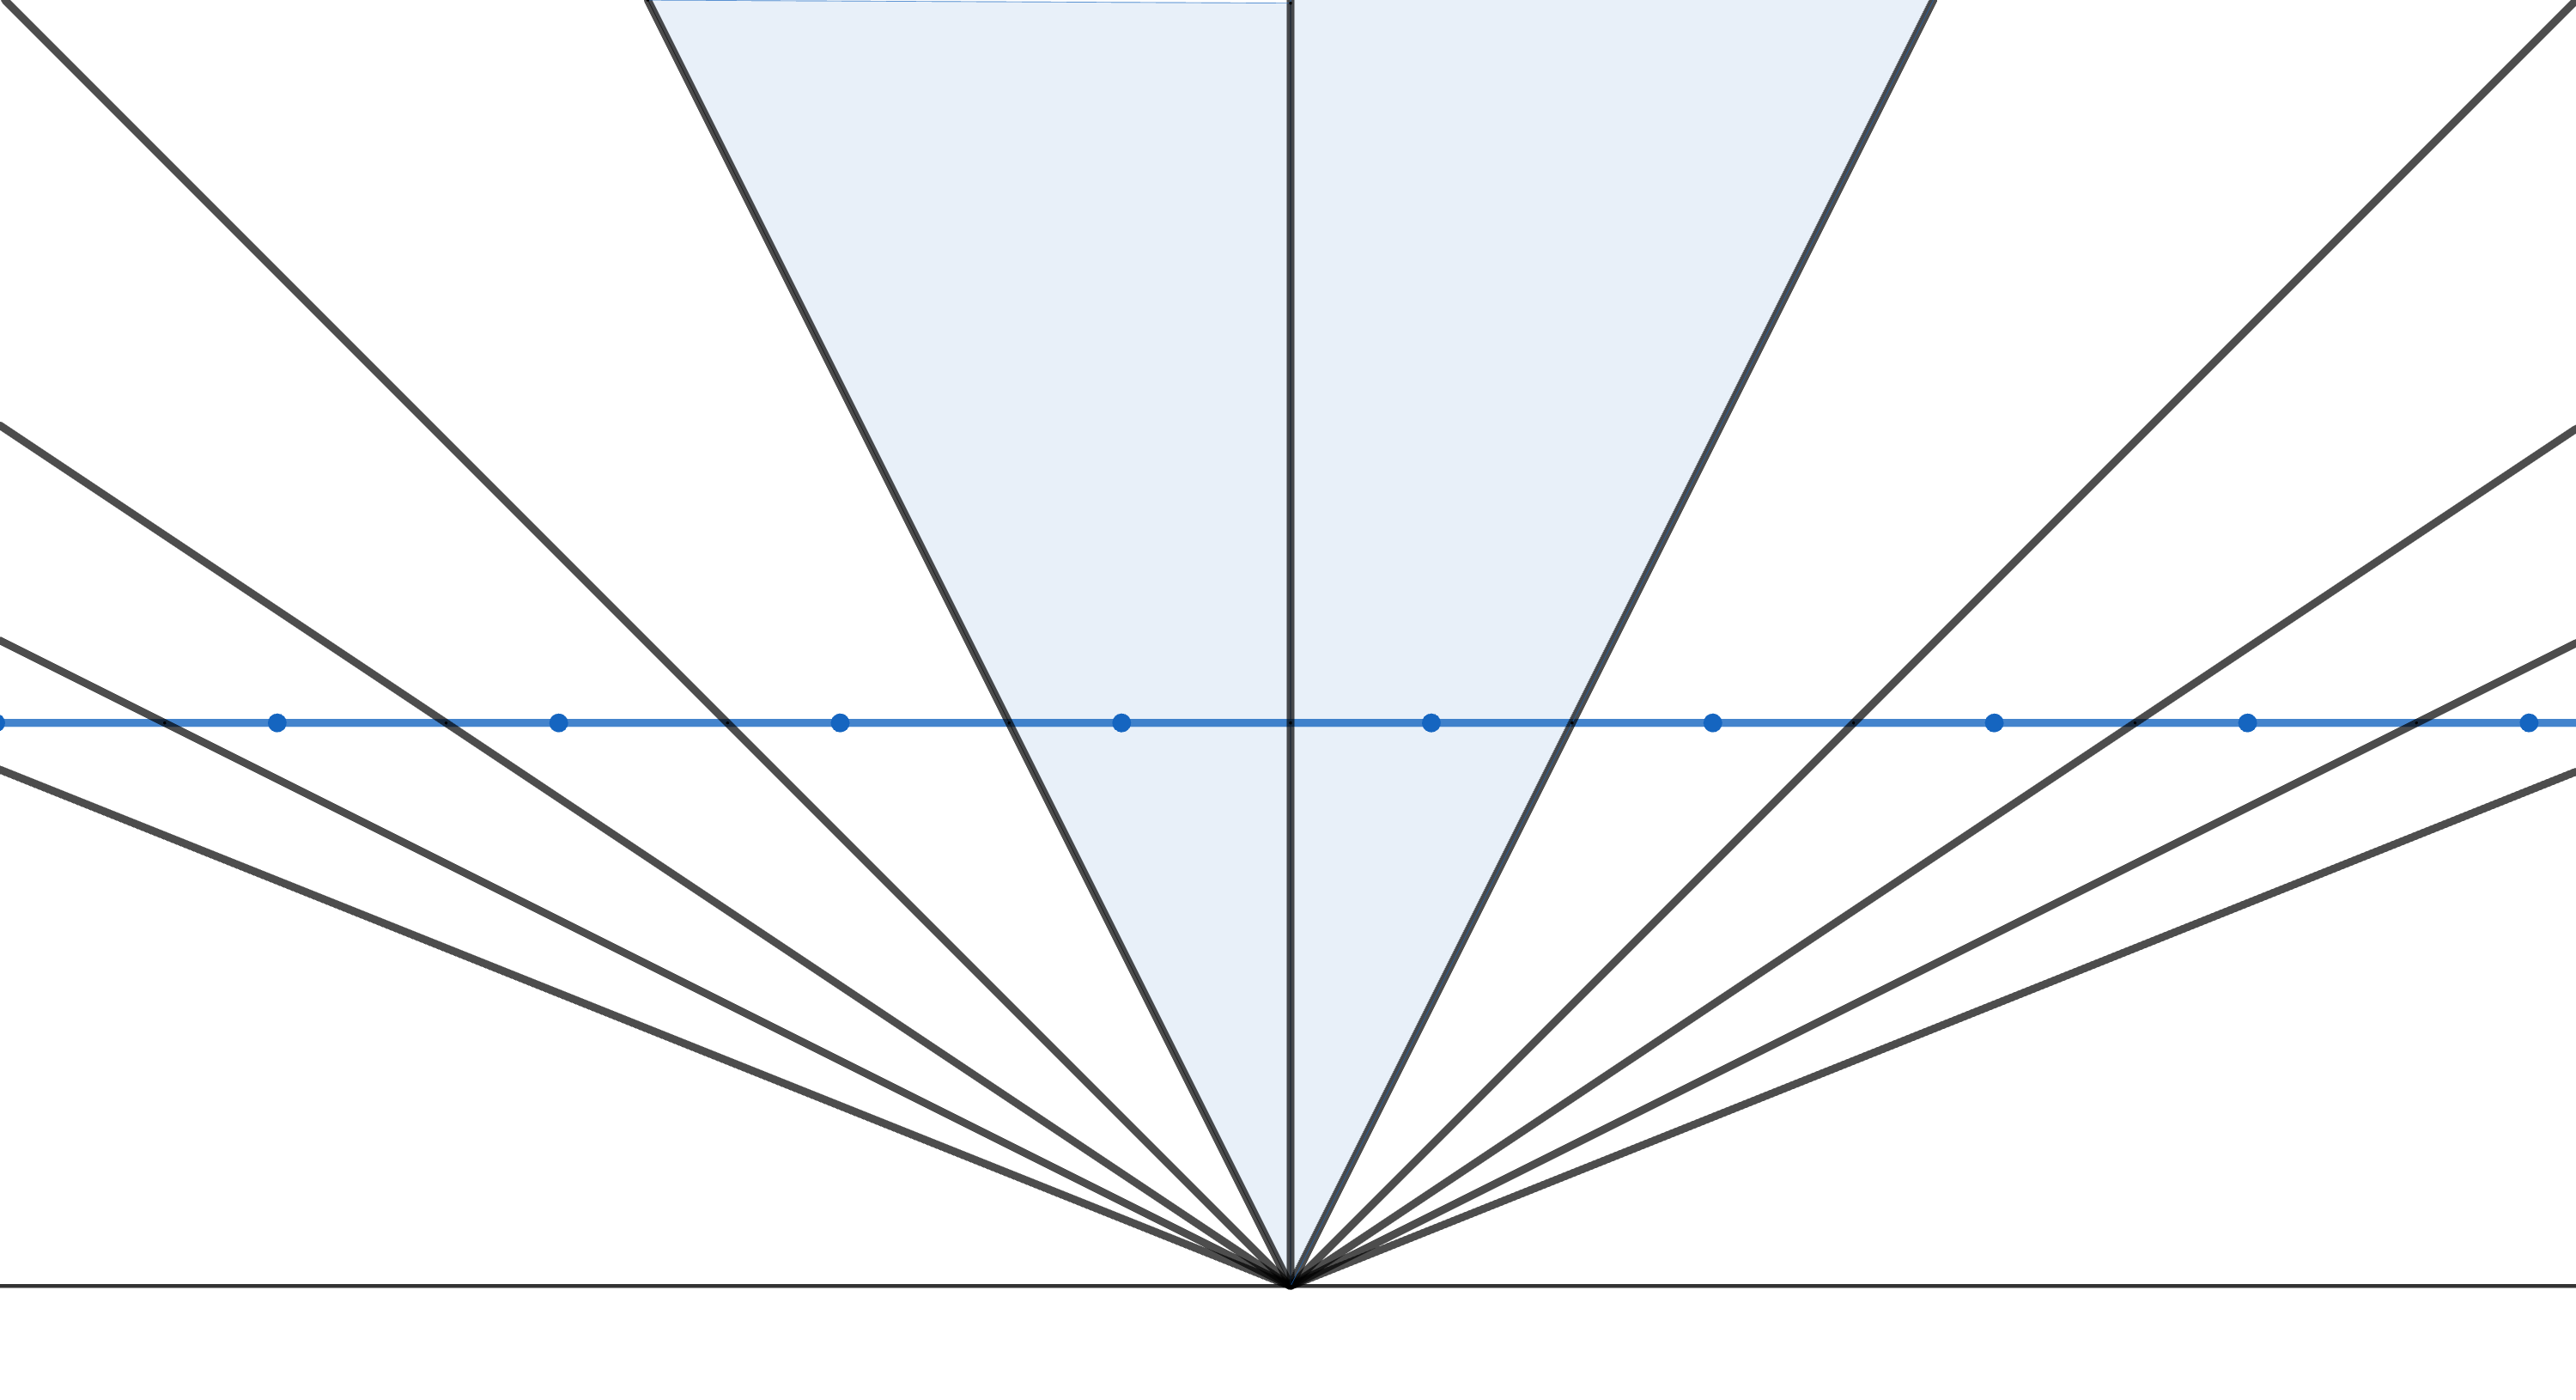
\includegraphics[width=6cm]{gfx/chamber graph - 2.png}}}\newline
%     \subfloat[The double polytope \(P' = P \cup s_1s_2s_1(P)\)]{{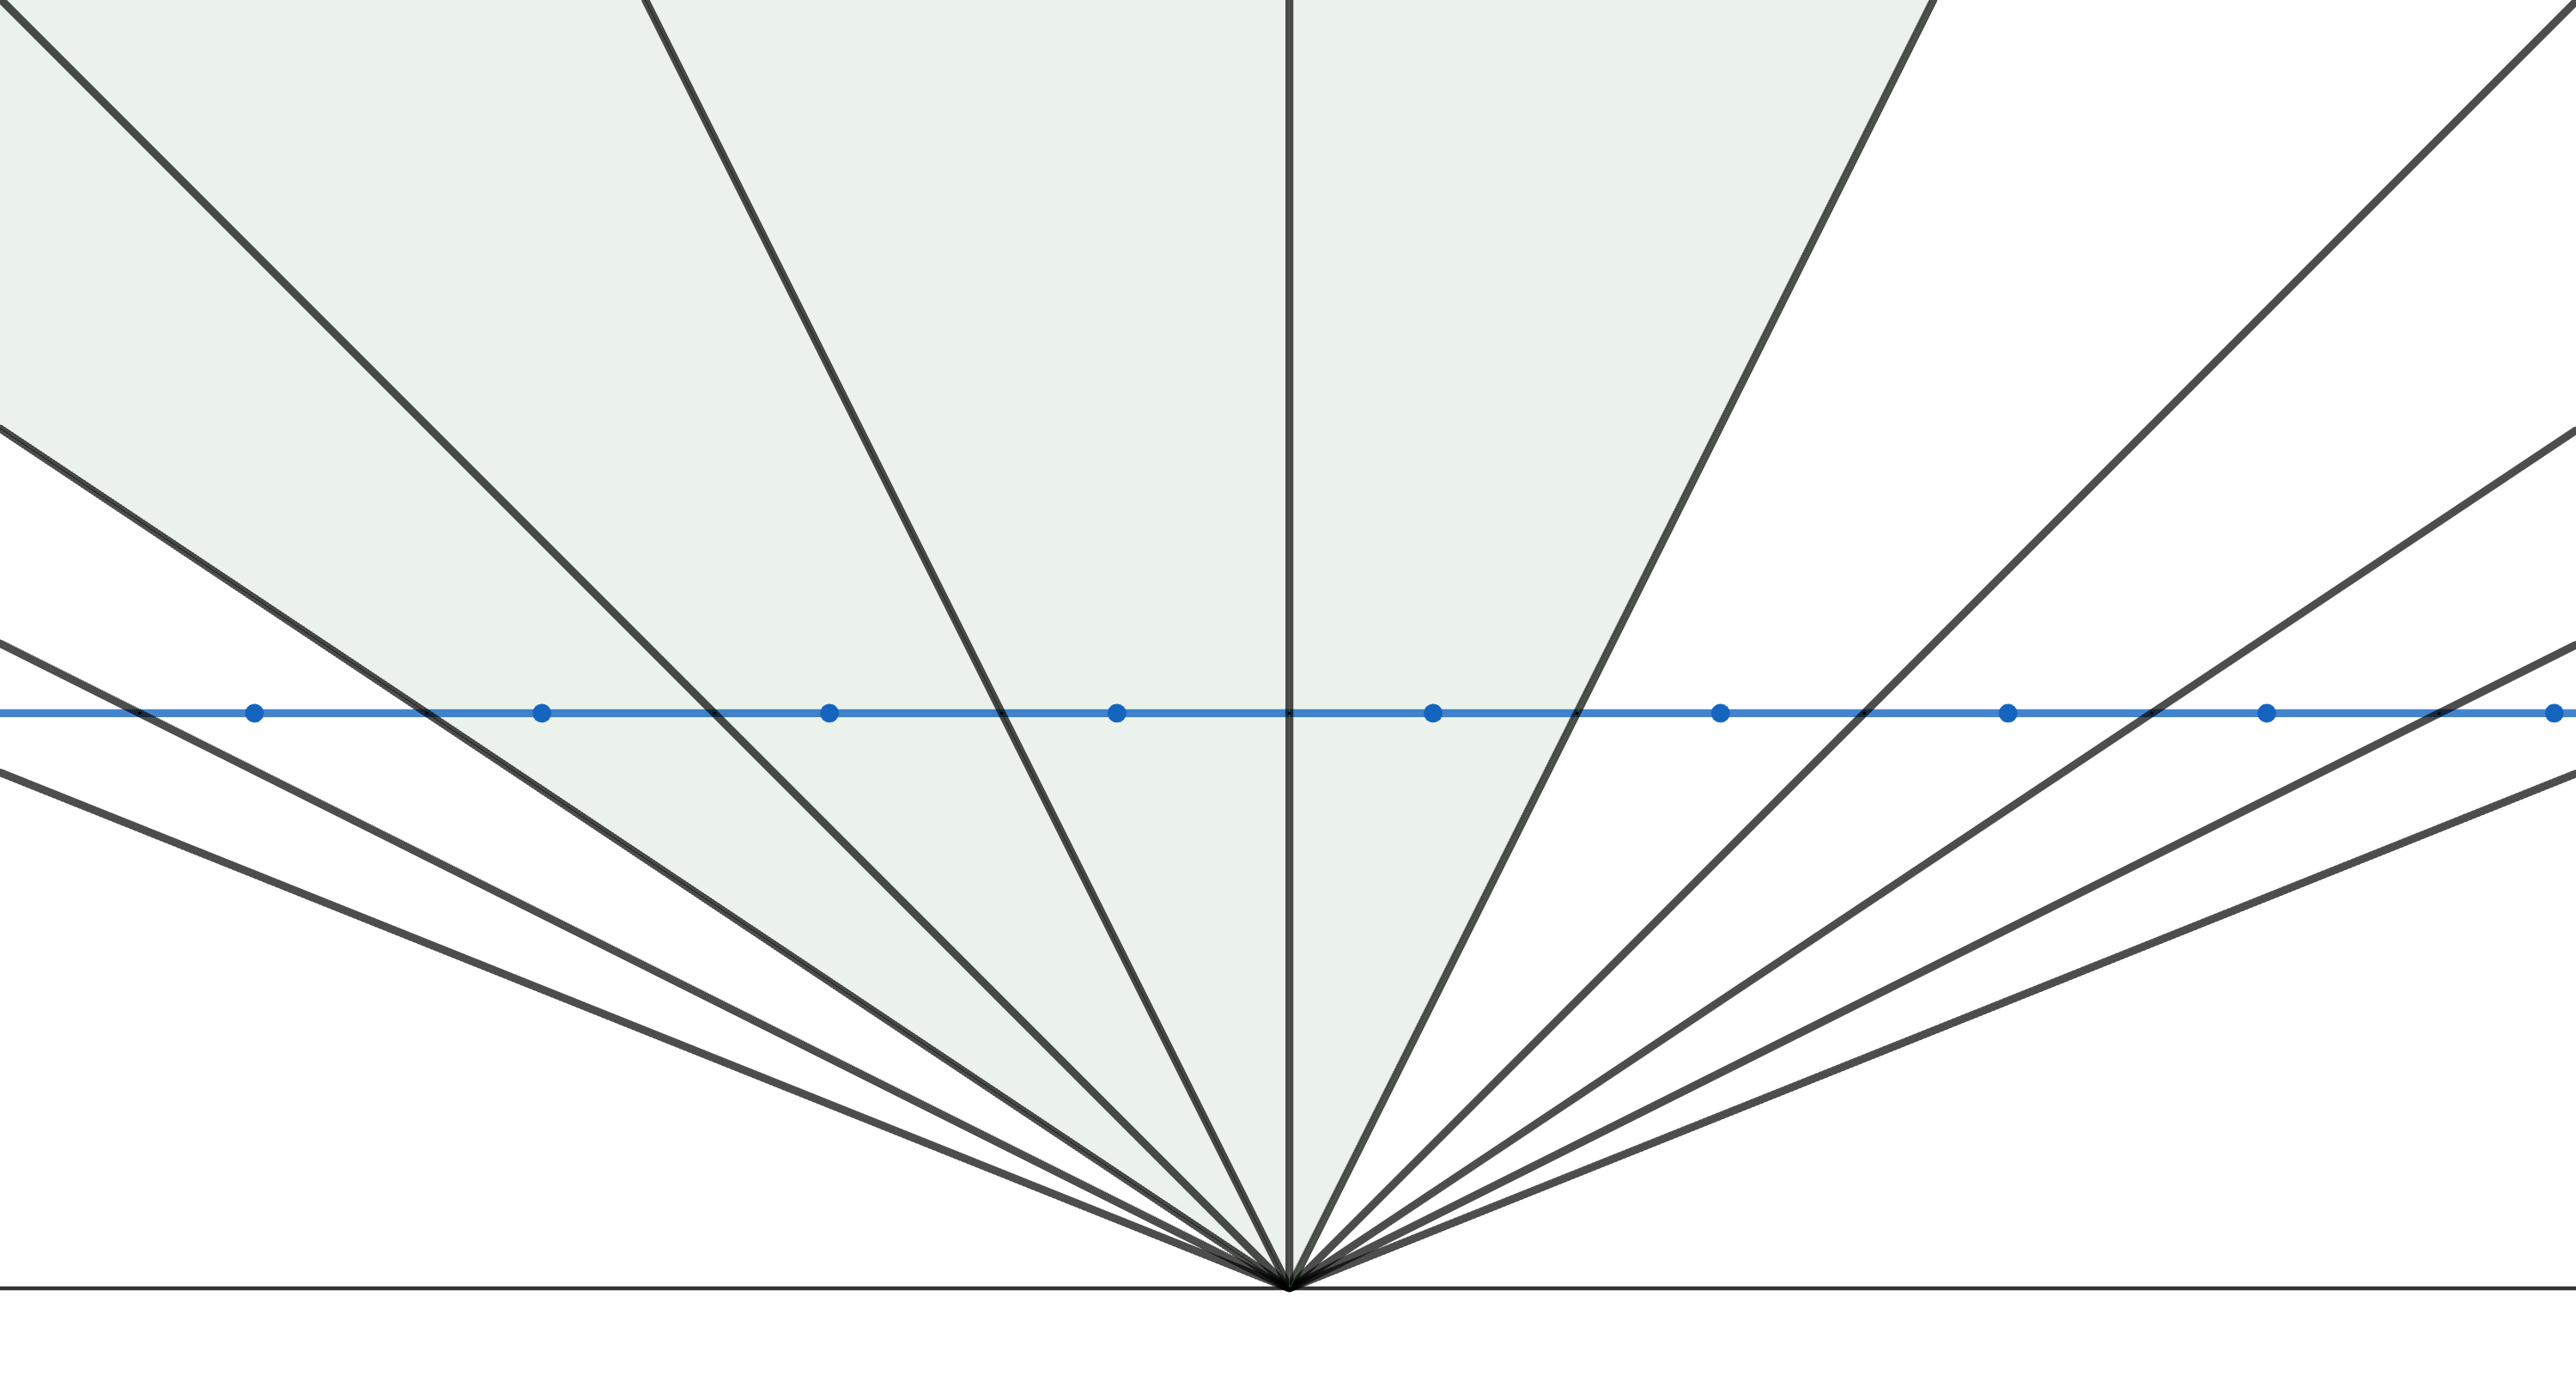
\includegraphics[width=6cm]{gfx/chamber graph - 3.png}}}
%     \caption{An example doubling sequence in \(D_\infty\)}
% \end{figure}

\newpage
% ***********************************************
\section{The manifold sequence}
% ***********************************************

We finally have developed enough tools, to construct the desired sequence of subgroups in \(W'\).
Following \Cref{thm:cofinal}, we fix a cofinal doubling sequence \(P_k\), starting in the fundamental chamber \(P_0 = C\) of \(W\), i.e. a cofinal sequence of two-fold orbifold covers \(C \leftarrow P_1 \leftarrow P_2 \leftarrow \cdots\).
Then, we define the groups \(W_i := \pi_1^{\text{orb}}(P_i) \cap W'\) for \(i \in \{0\} \cup \N\), each inducing a manifold via the quotient \(\faktor{WC}{W_i}\).
Clearly, each \(W_i\) is a subgroup of \(W'\) as well as it is a subgroup of the orbifold fundamental group of the polytope \(P_i\).
Using the theory of orbifold coverings, we observe that they form manifold covers of the polytopes \(P_i\). % = \faktor{WC}{\pi_1^{\text{orb}}(P_i)}\).
By \Cref{rmk:groupseries}, the cofinal two-fold tower induces a descending series of fundamental groups and intersecting them with \(W'\) will not allow them to grow.
Thus, the series formed by the \(W_i\) is again cofinal.

\noindent
We observe that, to show that \(W'\) is RFRS, it remains to show the following two conditions:
\begin{enumerate}
    \item each \(W_i\) has finite index in \(W'\) and
    \item \((W_i)_r^{(1)} := \ker\{W_i \to \Q \otimes_\Z (W_i)_{\text{ab}}\}\) is a subgroup of \(W_{i+1}\).
\end{enumerate}
The first condition is essentially a consequence of the fact that the series of orbifold fundamental groups has index two in each step.
To conclude, we prove the following lemma.

\begin{lemma}\label{lem:index}
    The homomorphism \(\phi : A := \faktor{W_i}{W_{i+1}} \to B := \faktor{\pi_1^{\text{orb}}(P_i)}{\pi_1^{\text{orb}}(P_{i+1})}\) is injective.
\end{lemma}
\begin{proof}
    Suppose, \(g,h \in A = \faktor{W_i}{W_{i+1}}\) with \(\phi(g) = \phi(h)\), which is equivalent to
    \[g \cdot \pi_1^{\text{orb}}(P_{i+1}) = h \cdot \pi_1^{\text{orb}}(P_{i+1}) \iff g^{-1}h \in \pi_1^{\text{orb}}(P_{i+1}).\]
    % But \(g, h \in \faktor{W_i}{W_{i+1}}\) and \(W_i = \pi_1^{\text{orb}}(P_{i+1}) \cap W'\) imply \(g^{-1}h = 1_A\) and thus, \(g = h \in A\).
    But the fact that \(g\) and \(h\) lie in \(\faktor{W_i}{W_{i+1}}\), and the definition of the groups \(W_i\) imply that \(g^{-1}h = 1\) in the quotient \(\faktor{W_i}{W_{i+1}}\).
    We conclude that \(g = h\) and the result follows. 
\end{proof}

An immediate consequence of this is the following result, we want to record here.

\begin{corollary}
    The index of \(W_{i+1}\) in \(W_i\) is less than or equal to \(2\).
\end{corollary}

% With this insight in hand, we are now able to conclude that the first of the remaining conditions is satisfied by the constructed series of groups.
Based on this observation, we can conclude that the first remaining condition holds for the constructed sequence of groups.
We state this here as a corollary as well.

\begin{corollary}
    The index of \(W_i\) in \(W'\) is finite.
\end{corollary}
\begin{proof}
    By the above corollary, we have that the index of \(W_{i+1}\) in \(W_i\) is less than or equal to \(2\).
    % As elaborated on in the beginning of this section, the \(W_i\) form a cofinal descending series of groups.
    % This allows us to conclude that for some \(n \in \N\), we have that \(W_j = \{1\}\) for all \(j \geq n\).
    Thus, for the index of \(W_i\) in \(W'\) we have the upper bound \([W':W_i] \leq 2 \cdot i < \infty\) for \(i \in \N\).
\end{proof}

Verifying the first condition was relatively straightforward.
However, the final one requires slightly more work.
We will address it in the last section.


% ***********************************************
\section{Loops bouncing off faces}
% ***********************************************

As discussed in previous section, we need to show that the rational derived group \((W_i)_r^{(1)}\) is a subgroup of \(W_{i+1}\).
First, recall the following result, addressing abelian quotients.

\begin{lemma}
    Let \(G\) be a group with normal subgroup \(N \triangleleft G\).
    The quotient group \(\faktor{G}{N}\) is abelian if and only if the derived subgroup \(G^{(1)} = [G, G]\) of \(G\) is contained in the normal subgroup \(N\).
\end{lemma}
\begin{proof}
    \begin{itemize}
        \item[`\(\Rightarrow\)'] As \(N\) is normal in \(G\) and the quotient is abelian, for any \(g,h \in G\) we have that
            \[ghN = gN \cdot hN = hN \cdot gN = hgN \iff g^{-1}h^{-1}gh \in N.\]
            This is equivalent to the commutator \([g, h]\) being in \(N\) for all \(g,h \in G\), therefore \([G, G] \subset N\).
        
        \item[`\(\Leftarrow\)'] As now, \([G, G] \subset N\) for any \(g \in G\) and \(n \in N\), we have
            \[gng^{-1} = gng^{-1}n^{-1}n = [g, n]n.\]
            Since \([G, G] \subset N\), this element is again in \(N\) so that \(N\) is normal in \(G\).
            To see that the quotient by \(N\) is abelian, we take \(g, h \in \faktor{G}{N}\) and calculate
            \[gN \cdot hN = ghN = hgg^{-1}h^{-1}ghN = hg[g^{-1}, h^{-1}]N = hgN = hN \cdot gN.\]
            The result follows directly.
    \end{itemize}\vspace*{-2\parskip}
\end{proof}

\noindent
Note that we have the situation that either the quotient \(\faktor{W_i}{W_{i+1}}\) is isomorphic to \(\faktor{\Z}{2\Z}\) or it is trivial, meaning that \(W_{i} = W_{i+1}\).
In particular, the quotient is abelian and we can apply the lemma above.
This tells us that the derived subgroup of \(W_i\) is contained in \(W_{i+1}\), i.e. in the kernel of the quotient homomorphism, which is normal in \(W_i\).
Stated differently, we have a factorization through the abelianization.

\noindent
Recall that torsion elements won't survive in the rational derived subgroup (cf. \Cref{rmk:tensoring}).
Thus, to show that the rational derived subgroup \((W_i)_r^{(1)}\) is a subgroup of \(W_{i+1}\), we have to show that each element \(g \in W_i\) with non-trivial image in the quotient \(\faktor{W_i}{W_{i+1}}\) is not torsion.
These elements will admit a factorization through the torsion-free abelianization as follows.
\begin{figure}[h!]
    \centering
    \begin{tikzcd}
        W_i \arrow[rr] \arrow[dr] & {} & \faktor{W_i}{W_{i+1}} \cong \faktor{\Z}{2\Z} \\
        {} & \faktor{(W_i)_{\text{ab}}}{\text{Torsion}} \arrow[ru, dashed]
    \end{tikzcd}
\end{figure}

With our goal in mind, we take an arbitrary element \(g\) in the group \(W_i\) that is not contained in \(W_{i+1}\), together with a loop \(\gamma\) that is a representative of \(g\).
Note that \(\gamma\) is a loop living in the manifold \(\faktor{WC}{W_i}\), covering the polytope \(P_i\).
To keep the notation more readable, we will denote these manifolds by \(M_i\) in the following.

\begin{remark}
    As we have to deal with quite a few objects in the following, we fix some notation.
    \begin{enumerate}
        \item The manifolds arising from the quotients \(\faktor{WC}{W_i}\) will be denoted \(M_i\),
        \item covering map \(p_i: M_i \to P_i\), will be shortly denoted by \(\pi_i\),
        \item the face of \(P_i\), in which gets doubled to obtain \(P_{i+1}\), will be denoted \(F_i\),
        \item in particular, the preimage of \(F_i\) is denoted \(p_i^{-1}(F_i)\).
    \end{enumerate}
\end{remark}

To see what is going on, we project \(\gamma\) down to \(P_i\) generically, using the covering map \(p_i\). %from \(M_i\) to \(P_i\).
As the polytope \(P_i\) has cyclic local group of order two everywhere on its codimension-\(1\) faces, what we see is a ray bouncing around the orbifold. % TODO: corner points!
One could think of a polytope with mirrors as faces and we are watching a ray of light getting reflected in the mirrors.
Now, fix the face \(F_i\) in which \(P_i\) is doubled to produce \(P_{i+1}\).
By our choice of \(g\), what we are seeing is that \(\gamma\) hits \(F_i\) an odd number of times.
If it would hit \(F_i\) an even number of times, \(\gamma\) would lift to a loop in \(P_{i+1}\) and therefore \(g\) would lift to \(W_{i+1}\), a contradiction.
In particular, observing the loop \(\gamma\) in the manifold \(M_i\), we see \(\gamma\) intersecting the preimage of \(F_i\) in \(M_i\) an odd number of times as well.

\begin{remark}
    We want to explain what is happening here in a more explicit way.
    To do so, we look at the following picture, which one should think of in a schematic way.
    We see a loop \(\gamma\) (which formally is the projection of a loop in \(M_i\)) in the polytope \(P_i\), being reflected in faces.
    The face of interest \(F_i\) is colored in blue and we assume \(\gamma\) to be the orange path, walked around exactly once, starting in the basepoint \(x_0\).
    \begin{figure}[h!]
        \label{fig:ray}
        \centering
        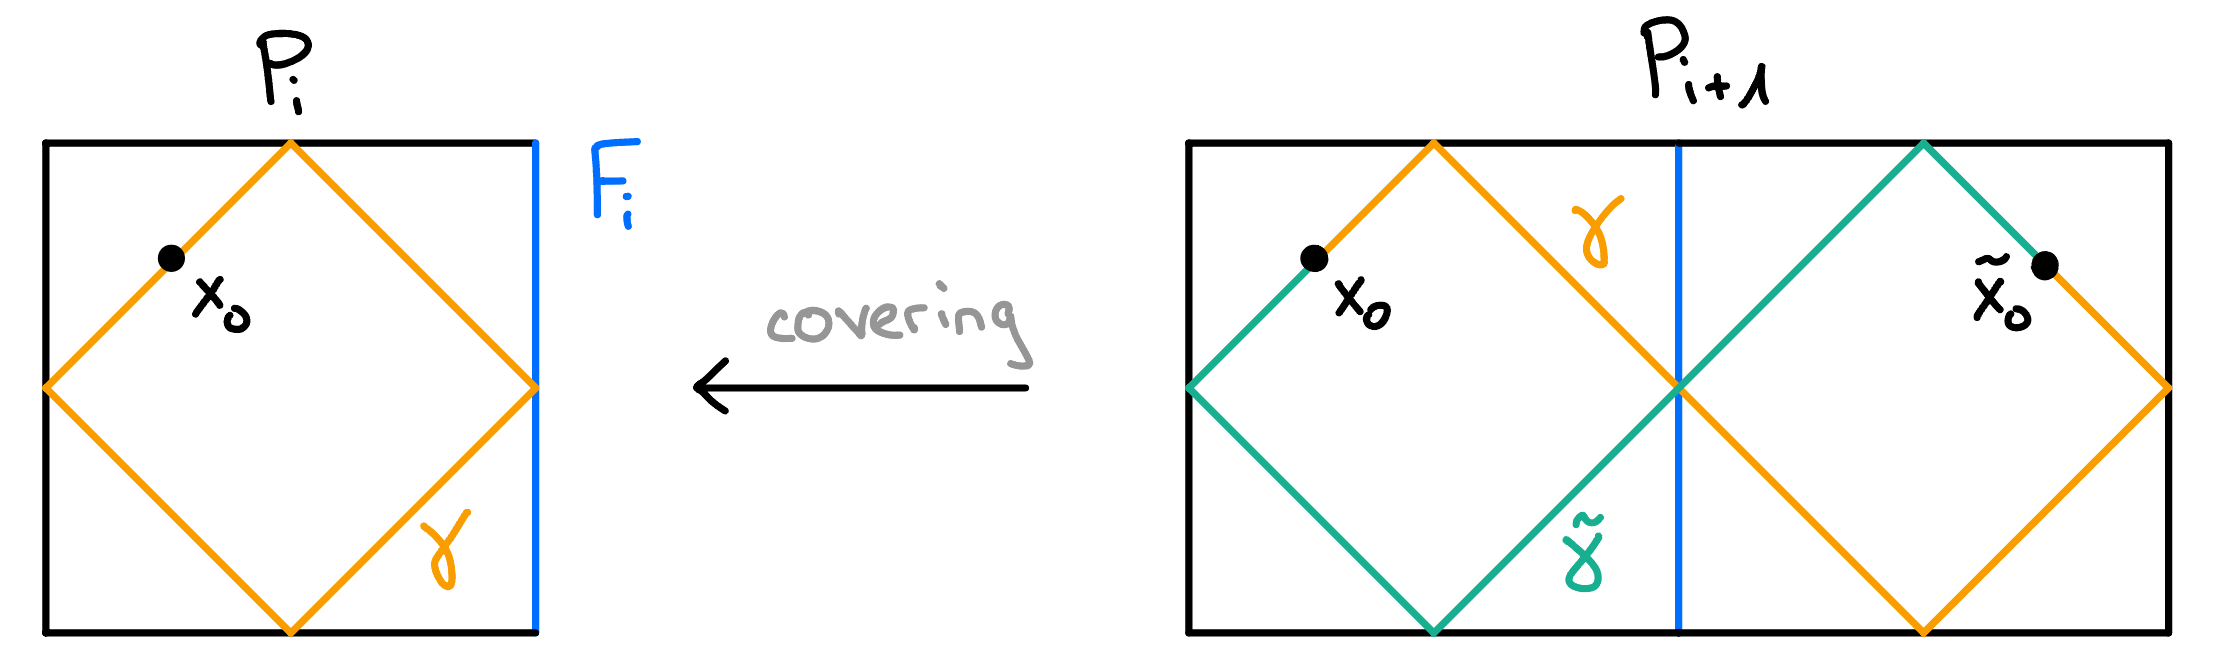
\includegraphics[width=.8\textwidth]{gfx/Ray bouncing in P.png}
    \end{figure}\vspace*{-\parskip}

    \noindent
    By doubling this polytope \(P_i\) along the face \(F_i\), we land on the right side of this picture.
    Observe that the basepoint \(x_0\) now has a corresponding double \(\widetilde{x}_0\).
    The more interesting part is, that now the loop \(\gamma\) gets unwound to a path going from \(x_0\) to \(\widetilde{x}_0\).
    On the other hand, if we consider the loop \(\gamma^2\), i.e. the loop \(\gamma\) gets run through twice, consequently hitting the face \(F_i\) twice.
    By our reasoning above, we should see a loop coming from \(\gamma^2\) in the two-fold cover \(P_{i+1}\).
    Indeed, the loop \(\gamma^2\) lifts to \(P_{i+1}\) and is pictured by the concatenated loop \(\widetilde{\gamma} \cdot \gamma\) in \(P_{i+1}\) on the right.
\end{remark}

Now that we have a more intuitive view on our reasoning, we have to deal with one more minor issue.
We will mention it in the following remark, but will omit the details.

\newpage
\begin{remark}
    Note that we could also have a loop \(\gamma\) like in the left of the following image.
    \begin{figure}[h!]
        \label{fig:badray}
        \centering
        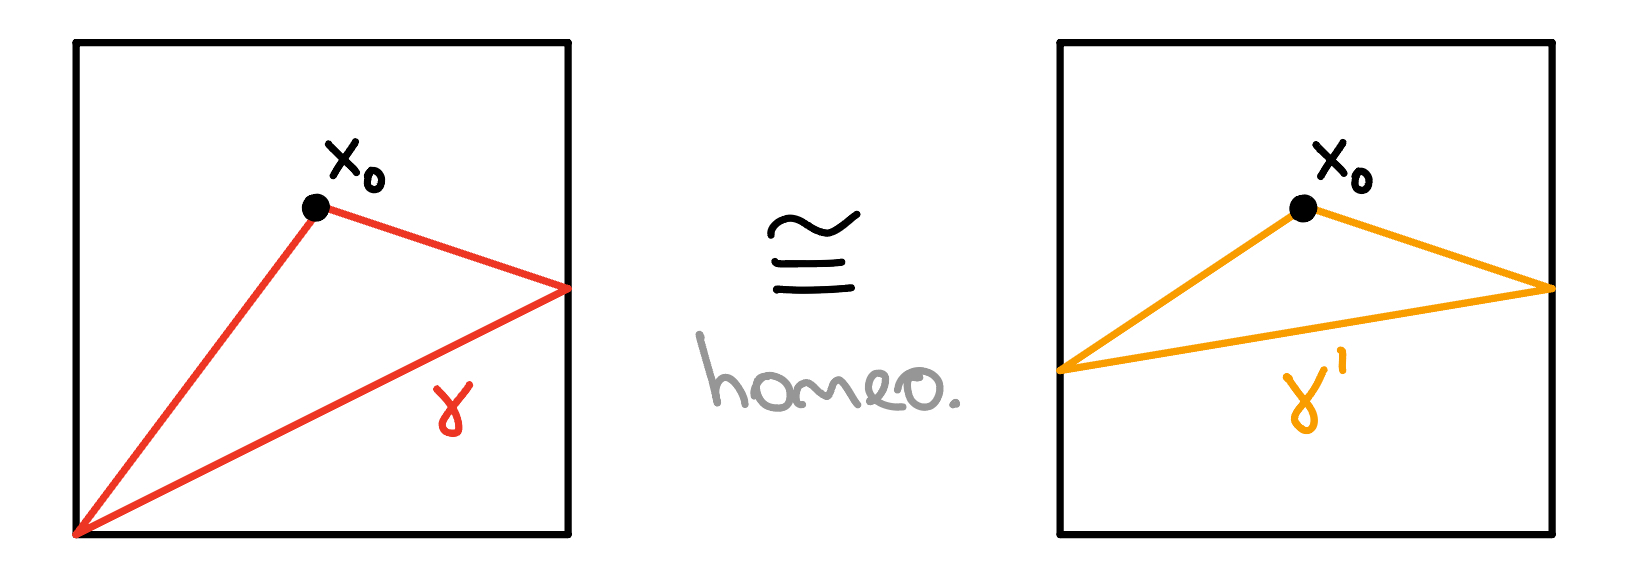
\includegraphics[height=3.2cm]{gfx/Equivalent loops.png}
    \end{figure}\vspace*{-\parskip}

    \noindent
    The difficulty with such loops is that the codimension-\(2\) faces of a polytope also consist of singular points.
    Their local group may very well be different from the local groups of the points in codimension-\(1\) faces.
    Nevertheless, we fortunately do not have to deal with them.
    In fact, we can always find a loop \(\gamma'\), homotopy equivalent to \(\gamma\) and that is only hitting codimension-\(1\) faces.
\end{remark}

% Up to this point we have set up the stage for the next argument to fulfill the proof.

To see that the loop \(\gamma\) represents an element of infinite order in \(W_i\), we will construct a morphism of fundamental groups.
Namely, from the fundamental group \(\pi_1(M_i)\) of the manifold \(M_i\) to the fundamental group of the circle \(\pi_1(S^1)\).
If \(\gamma\) maps non-trivially to \(\pi_1(S^1)\), it has to represent an element of infinite order, as \(\pi_1(S^1) \cong \Z\).

A fact we have not mentioned yet is that the preimage of a face \(F_i\) in the manifold \(M_i\) is two-sided.
This is a technical condition on the preimage \(p_i^{-1}(F_i)\), but it will be important in the following.
We give the definition.

\begin{definition}
    Let \(M\) be a manifold and \(F \subset M\) be a submanifold.
    Then, \(F\) is called \emph{two-sided} in \(M\), if it locally looks like the product with an intervall.
    More precisely, there is a neighborhood \(N_F\) with \(N_F \cong F \times (-\varepsilon, \varepsilon)\) for suitable \(\varepsilon > 0\), where \(F\) is identified with \(F \times \{0\}\).
\end{definition}

The generic projection of \(\gamma\) down to the orbifold \(P_i\) implies that in the projection of the neighborhood \(N_{F_i}\), coming from the two-sidedness, the ray \(\gamma\) is injective, i.e. we don't just walk up to the face and go back without getting reflected. % TODO: check this!
As a consequence, in the manifold \(M_i\), the ray \(\gamma\) has to really intersect the preimage of \(F_i\).
We will now proceed by defining an equivalence relation on points in \(M_i\) as follows.
\begin{equation*}
    x \sim y  \qquad :\iff \qquad x, y \in M_i \backslash N_{F_i} \quad\text{or}\quad x = y.
\end{equation*}
% By passing to the quotient \(\faktor{M_i}{\sim}\), we collapse the endpoints of the closure \(\overline{N} \cong F_i \times [-\varepsilon, \varepsilon]\).
% Now, further collapse the single fibers \(F_i \times \{z\}\) for all \(z\) in the open interval \((-\varepsilon, \varepsilon)\).
% What we visually see, already is the one-dimensional sphere \(S^1\).
% We already mentioned that the generic projection implies that \(\gamma\) is injective in this neighborhood \(N\).
% This implies that \(\gamma\) actually intersects the face \(F_i\).
We now want to describe the space, arising by collapsing the manifold \(M_i\) relative to this equivalence relation, i.e. the quotient space \(\faktor{M_i}{\sim}\).
As all the points outside the neighborhood \(N_{F_i}\) get identified, we see a double cone with identified cone points.
\begin{figure}[h!]
    \label{fig:doublecone}
    \centering
    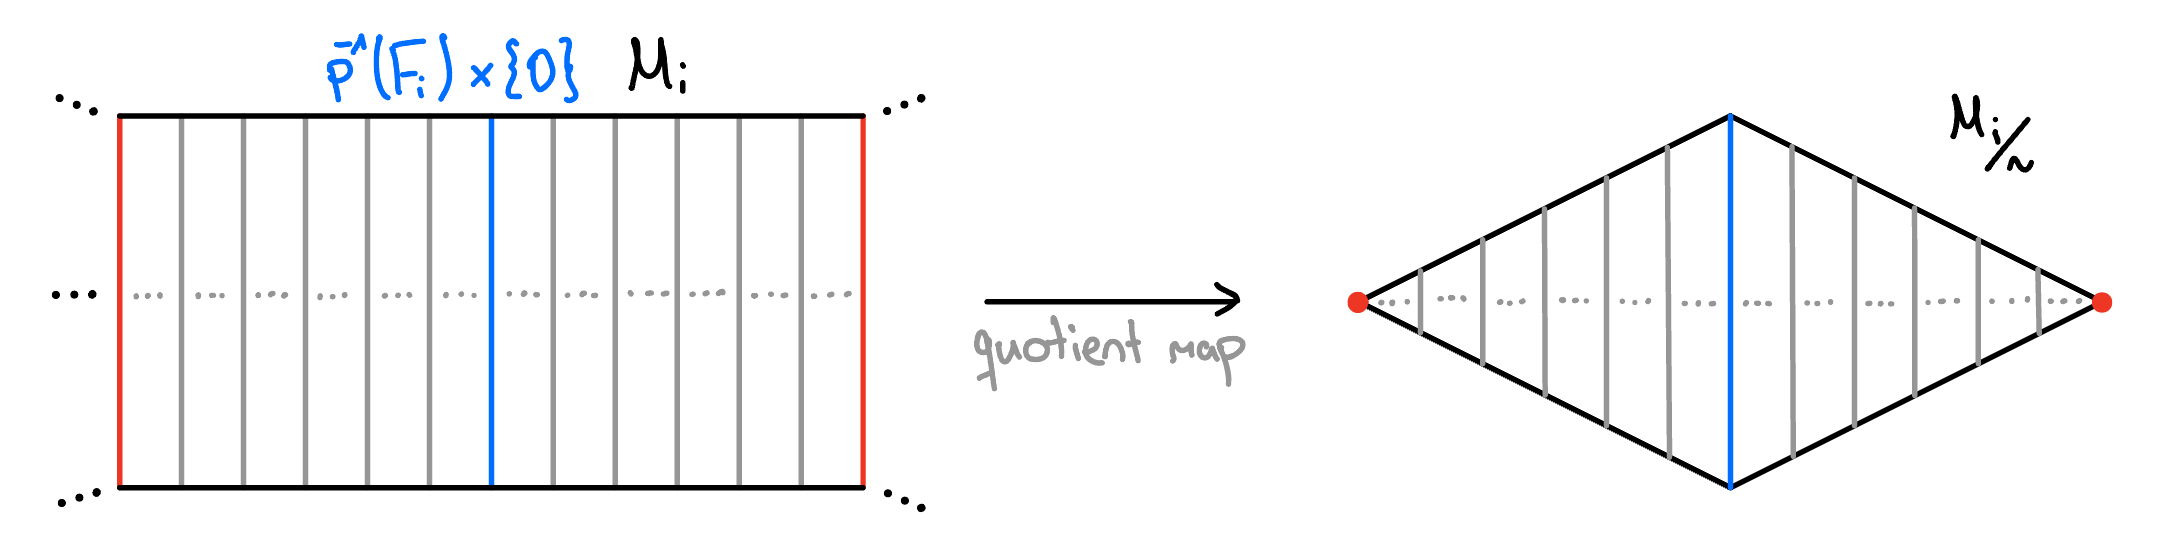
\includegraphics[width=.8\textwidth]{gfx/Quotient 1.png}
\end{figure}

This does not yet yield the desired morphism of fundamental groups.
We have to pass to another quotient by collapsing the `fibers' \(p_i^{-1}(F_i) \times \{z\}\) at every point \(z\) in the open interval \((-\varepsilon, \varepsilon)\), to a single point.
We receive the following picture.
\begin{figure}[h!]
    \label{fig:circle}
    \centering
    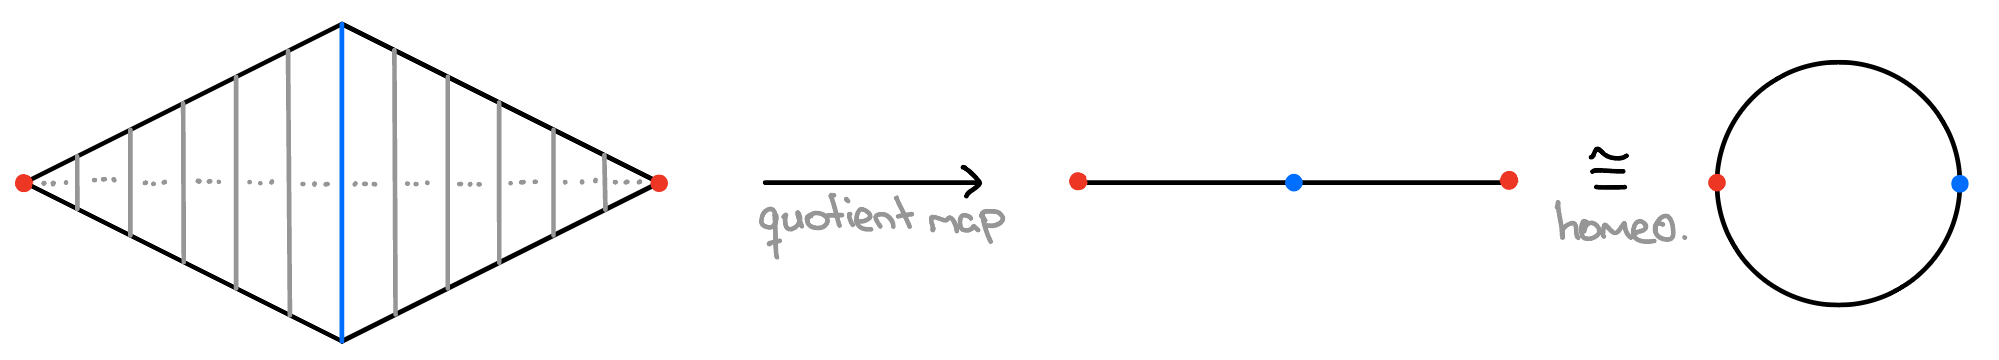
\includegraphics[width=.9\textwidth]{gfx/Quotient 2.png}
\end{figure}

By the way we think about quotient spaces, we already see that this results in \(S^1\).
